% !TEX root = ../../main.tex
\section{Artificial data generation}\label{sec:artificial_data_generation}
In this section we present four data sets, as used by Camci~\cite{camci2010change} and Takeuchi and Yamanishi \cite{takeuchi2006unifying}, to provide for a objective performance comparison.
All the data sets are modeled by a second-order \gls{ar}-model as in \Cref{eq:artificial_data_sets_model}, where $\epsilon_t$ is a Gaussian distribution modeling the noise with mean $0$ and variance $\sigma^2 = 1$, $a_1 = 0.6$ and $a_2 = -0.5$.
\begin{equation}\label{eq:artificial_data_sets_model}
  x_t = a_1 x_{t-1} + a_2 x_{t-2} + \epsilon_t,
\end{equation}
The length of $x_t$ is $10000$ and change points are generated at each $y \times 10000^\text{th}$ data point, with $y = (1, 2, 3, \dots, 9)$.

Using this general \gls{ar}-model, we create four different data sets, all visualized in \Cref{fig:plots_artificial_data_sets}.
Each data set is characterized by a change in mean, variance, or both in the Gaussian term $\epsilon_t$:
\begin{enumerate}
  \item \textbf{Fixed increasing mean:} at each change point $y$ the mean is increased with $\Delta(y) = 5$.
  This set is the first data set of Camci~\cite{camci2010change}.
  The main characteristic is that the difference between the means of the Gaussian term $\epsilon_t$ is fixed and thus the relative distance becomes smaller.
  The data is plotted in \Cref{fig:camci_fixed_increasing_mean}.

  \item \textbf{Reduced increasing mean:} at each change point $y$ the mean is increased with $\Delta(y) = 10 - y$.
  This set is the first data set of Takeuchi and Yamanishi~\cite{takeuchi2006unifying}.
  In contrast with the previous set, in this set the absolute difference in mean is reduced over time.
  The data is plotted in \Cref{fig:takeuchi_reduced_increasing_mean}.

  \item \textbf{Reduced increasing mean, increasing variance:} at each change point $y$ the mean is increased with $\Delta(y) = 10 - y$ and the standard deviation is of $\epsilon_t$ is $0.1 / (0.01 + (10000 - x)/1000)$.
  This set is the second set of Camci~\cite{camci2010change}.
  This set combines the reduced increasing mean property of the previous set with an increasing variance, causing the change points to become more vague over time.
  The data is plotted in \Cref{fig:camci_reduced_increasing_mean_increasing_variance}.

  \item \textbf{Alternating variance:} at each change point $y$ the variance $\sigma^2$ is set to $9.0$ when $y$ is odd, and to $1.0$ otherwise.
  This set is the thirds sets from Camci~\cite{camci2010change} and Takeuchi and Yamanishi~\cite{takeuchi2006unifying}.
  This data set is used to measure the ability of detecting changes in decrease of variance, as Camci~\cite{camci2010change} claims is not trivial.
  The data is plotted in \Cref{fig:camci_takeuchi_alternating_variance}.
\end{enumerate}

\begin{figure}
  \centering
  \begin{subfigure}[b]{1\textwidth}
   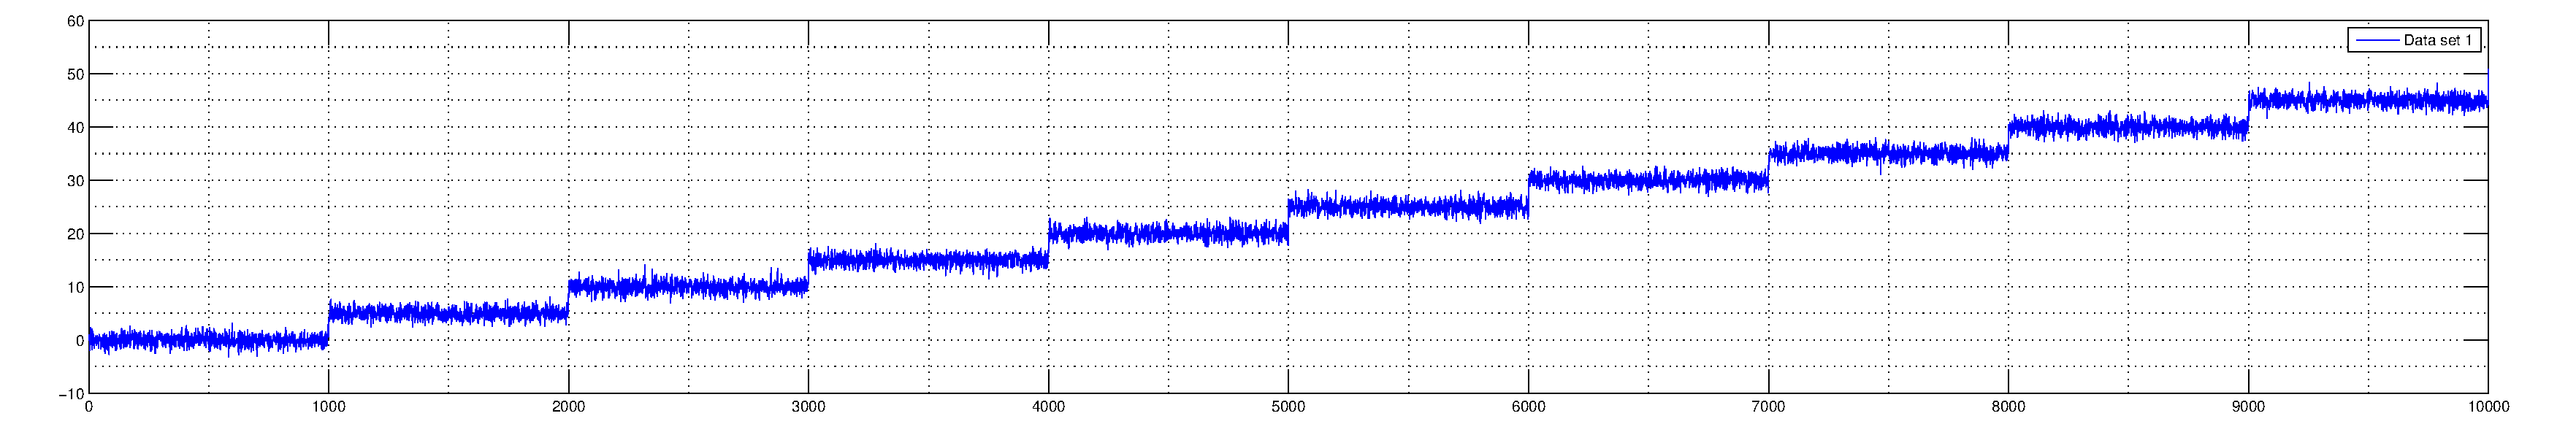
\includegraphics[width=1\textwidth]{./Figures/chapter5/set_1_data.eps}
   \caption[Fixed increasing mean]{Data set 1, \emph{Fixed increasing mean}.}
   \label{fig:camci_fixed_increasing_mean}
  \end{subfigure} \\

  \begin{subfigure}[b]{1\textwidth}
   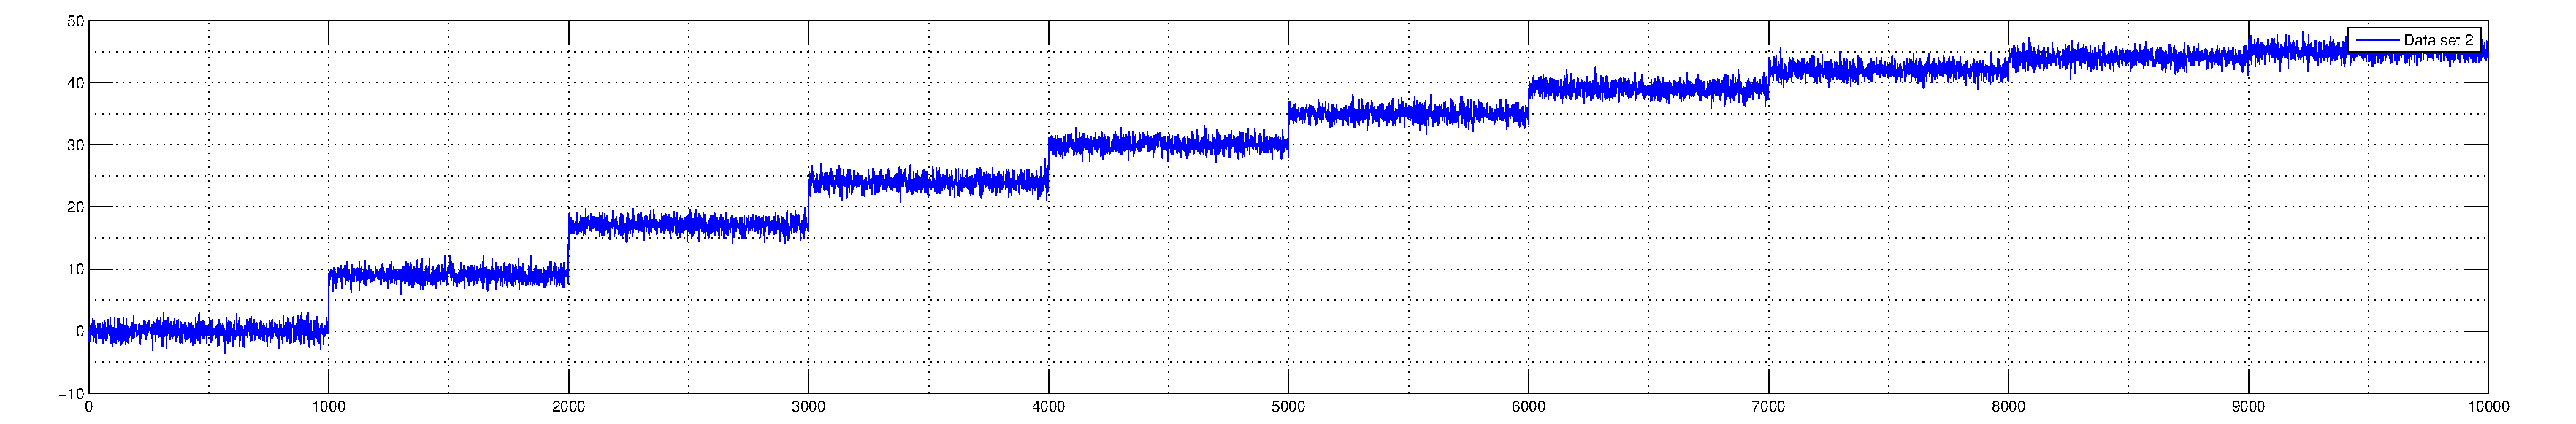
\includegraphics[width=1\textwidth]{./Figures/chapter5/set_2_data.eps}
   \caption[Reduced increasing mean]{Data set 2, \emph{Reduced increasing mean}.}
   \label{fig:takeuchi_reduced_increasing_mean}
  \end{subfigure} \\

  \begin{subfigure}[b]{1\textwidth}
    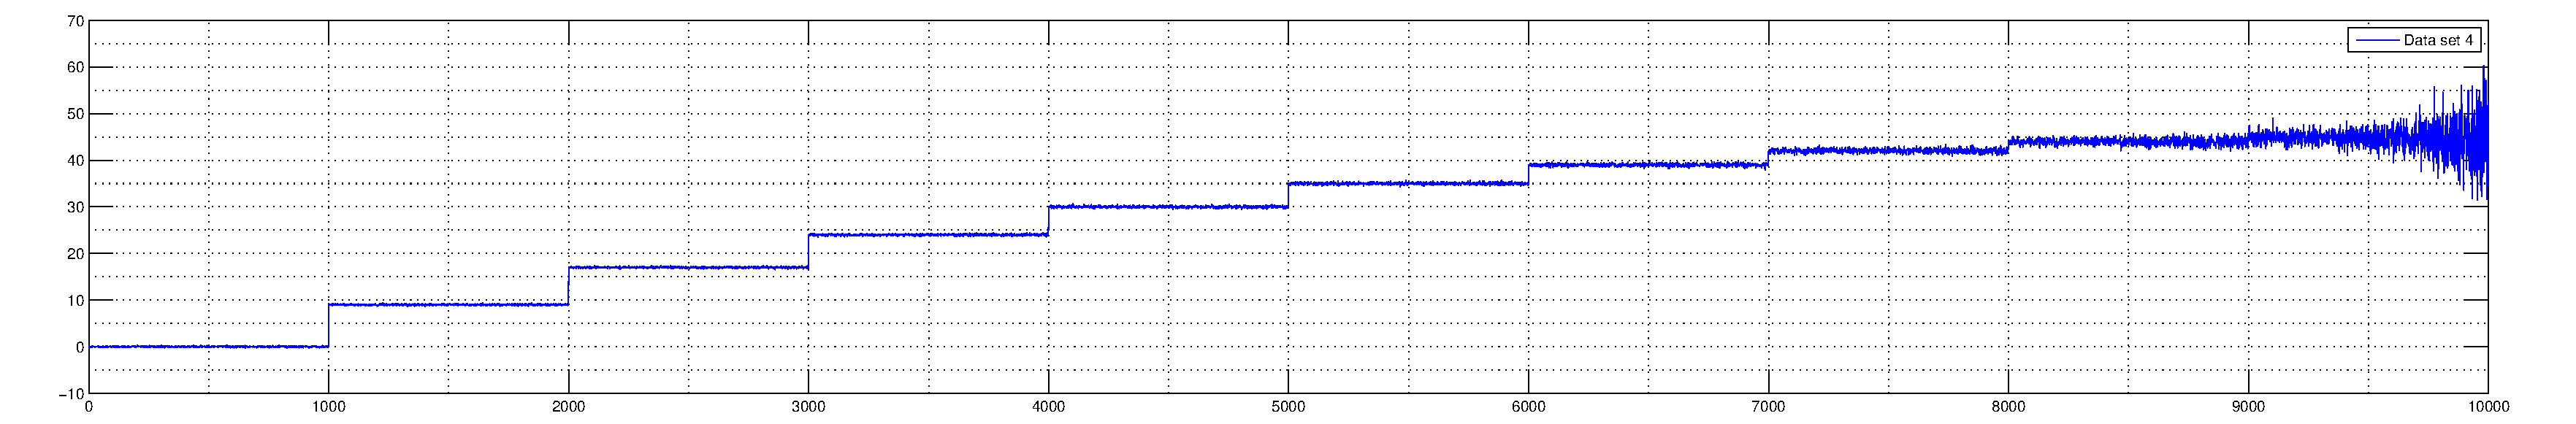
\includegraphics[width=1\textwidth]{./Figures/chapter5/set_3_data.eps}
    \caption[Reduced increasing mean, increasing variance]{Data set 3, \emph{Reduced increasing mean, increasing variance}.}
    \label{fig:camci_reduced_increasing_mean_increasing_variance}
   \end{subfigure} \\

  \begin{subfigure}[b]{1\textwidth}
   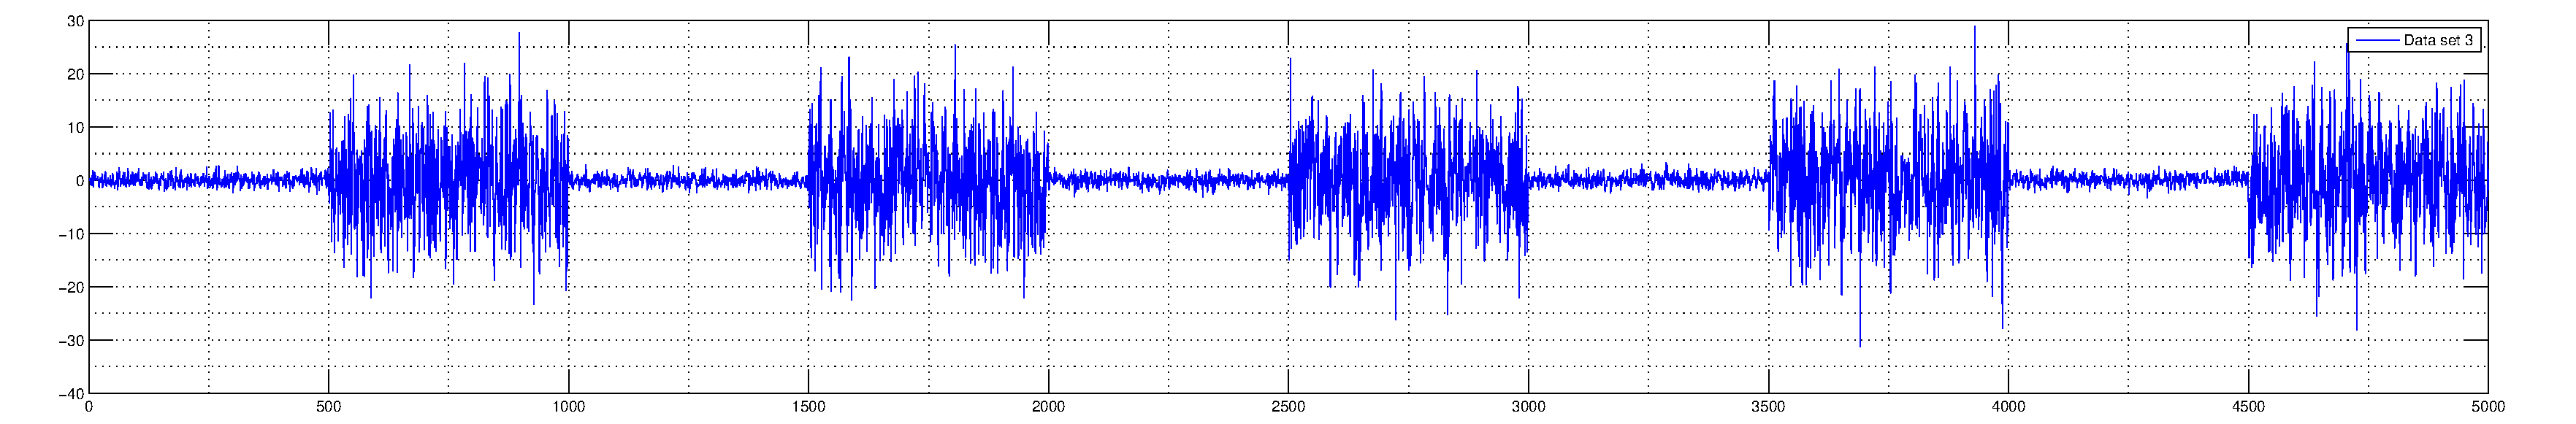
\includegraphics[width=1\textwidth]{./Figures/chapter5/set_4_data.eps}
   \caption[Alternating variance]{Data set 4, \emph{Alternating variance}.}
   \label{fig:camci_takeuchi_alternating_variance}
  \end{subfigure} \\

  \caption[Artificial data sets]{Plots of the artificial data sets used.}
  \label{fig:plots_artificial_data_sets}
\end{figure}



% \begin{figure}
% \centering
%   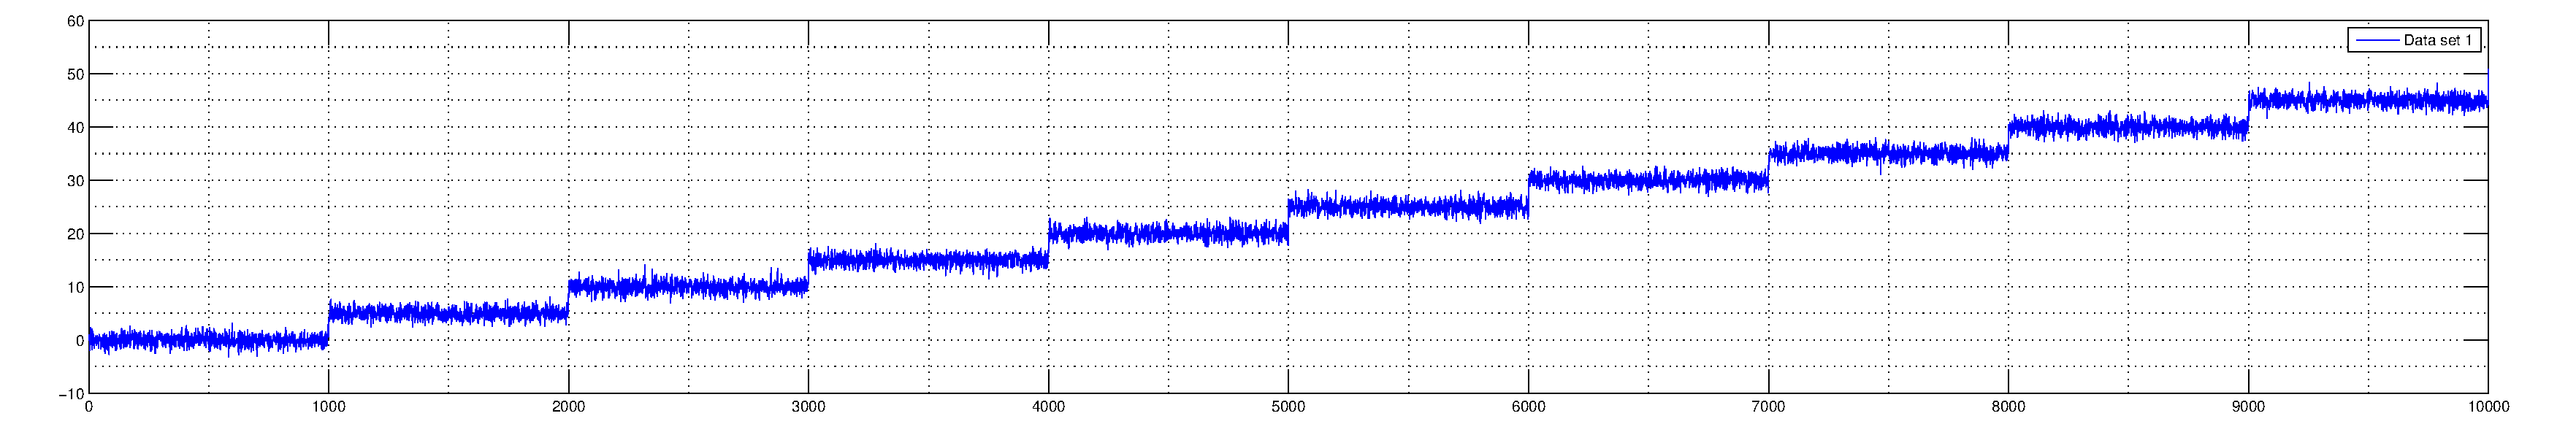
\includegraphics[width=1\textwidth]{./Figures/chapter5/set_1_data.eps}
%   \caption[Fixed increasing mean]{Data set 1, \emph{Fixed increasing mean}.}
%   \label{fig:camci_fixed_increasing_mean}
% \end{figure}

% \begin{figure}
% \centering
%   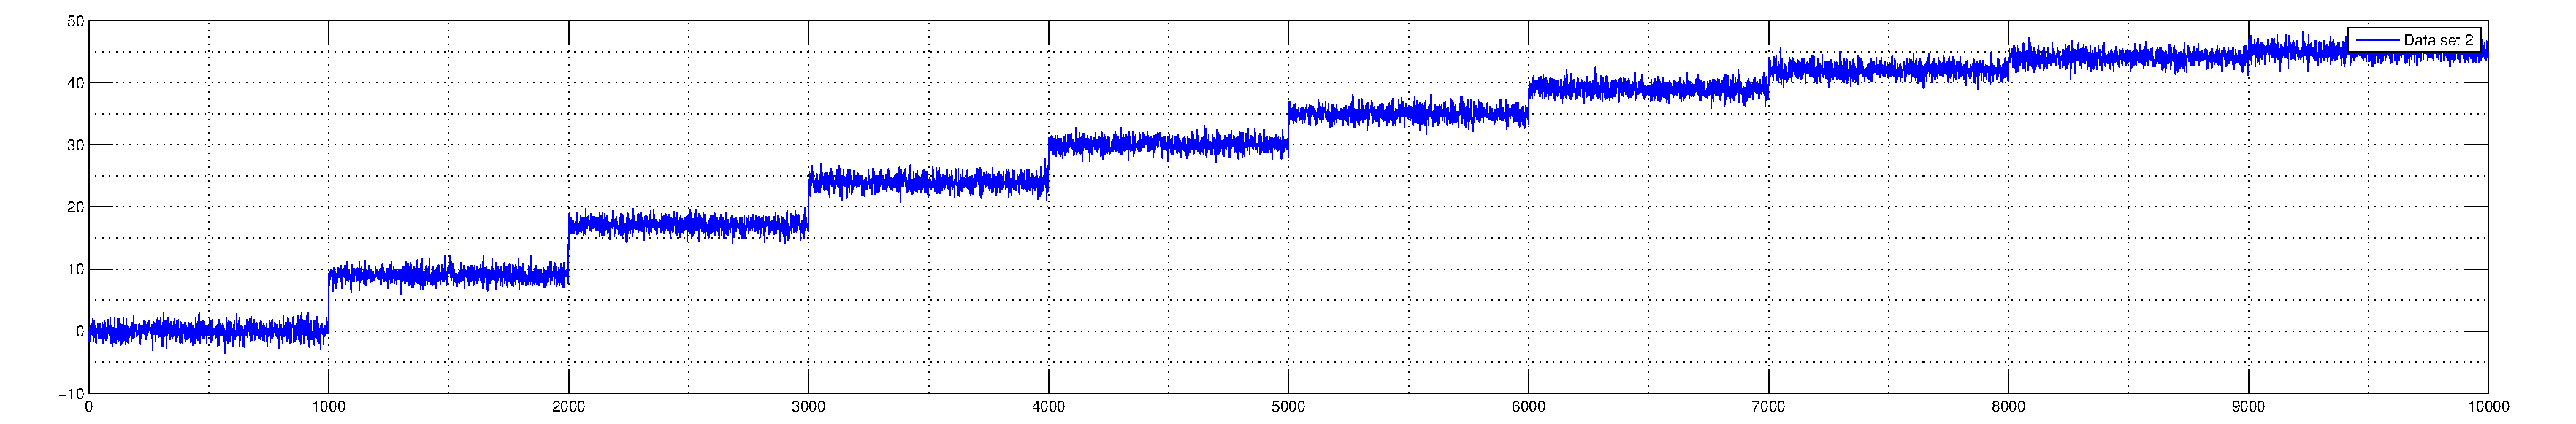
\includegraphics[width=1\textwidth]{./Figures/chapter5/set_2_data.eps}
%   \caption[Reduced increasing mean]{Data set 2, \emph{Reduced increasing mean}.}
%   \label{fig:takeuchi_reduced_increasing_mean}
% \end{figure}

% \begin{figure}
% \centering
%   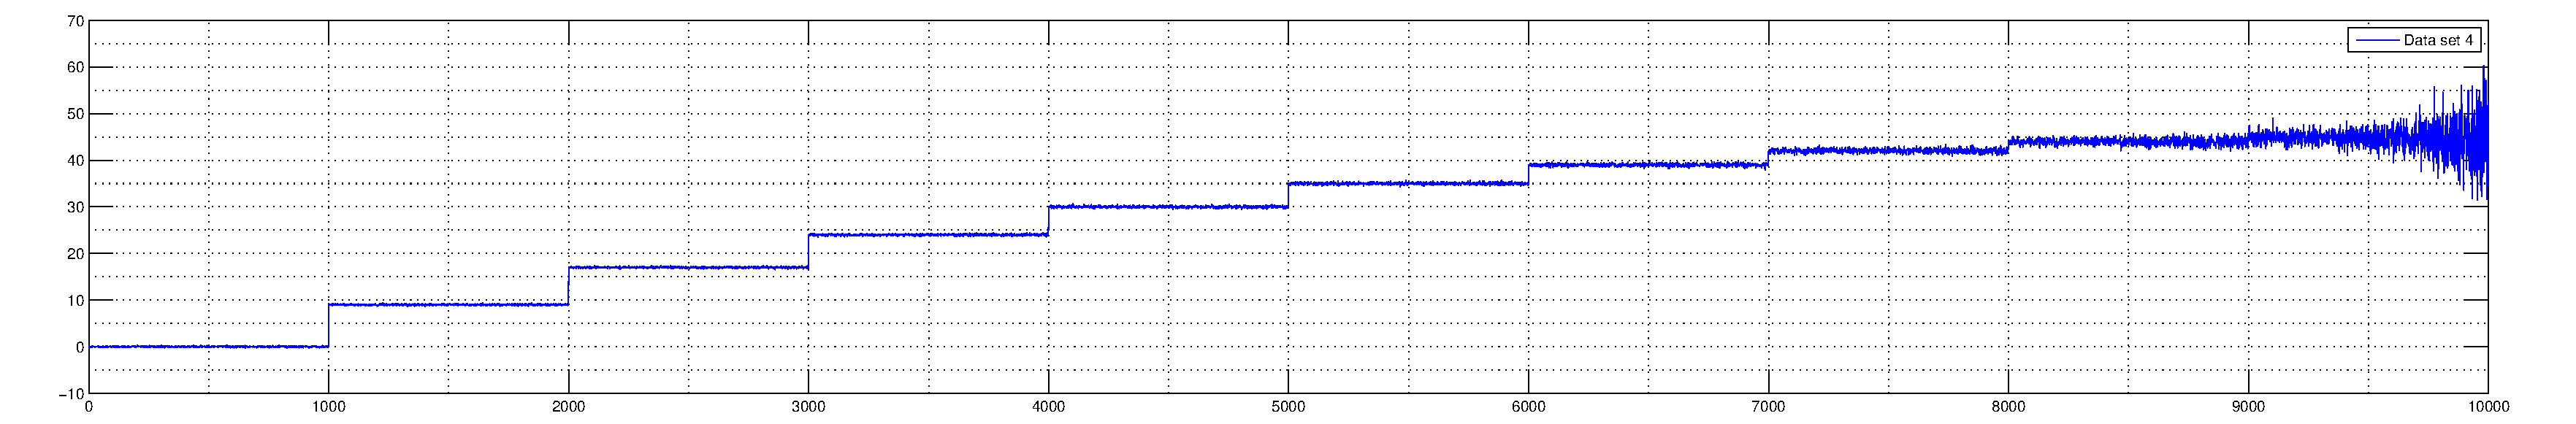
\includegraphics[width=1\textwidth]{./Figures/chapter5/set_3_data.eps}
%   \caption[Reduced increasing mean, increasing variance]{Data set 3, \emph{Reduced increasing mean, increasing variance}.}
%   \label{fig:camci_reduced_increasing_mean_increasing_variance}
% \end{figure}

% \begin{figure}
% \centering
%   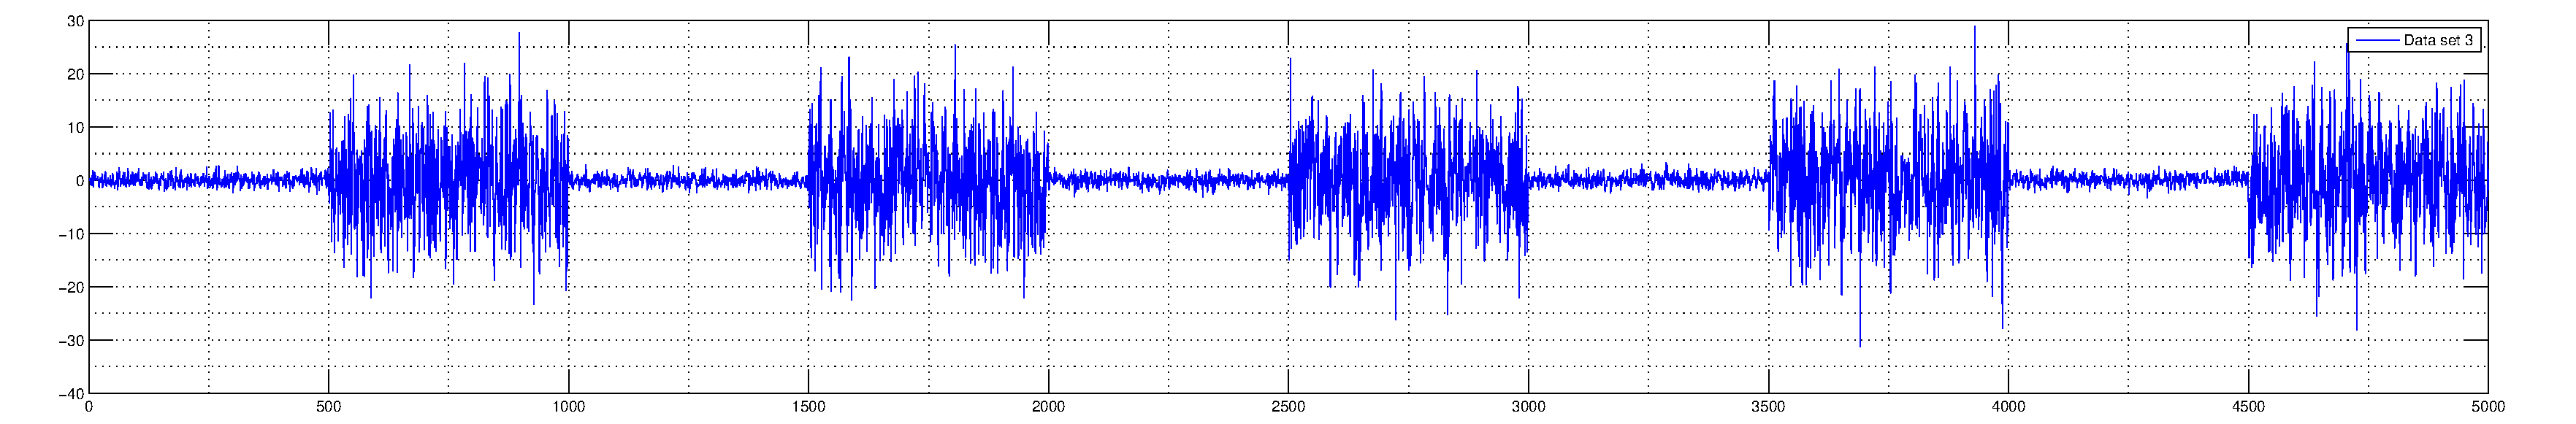
\includegraphics[width=1\textwidth]{./Figures/chapter5/set_4_data.eps}
%   \caption[Alternating variance]{Data set 4, \emph{Alternating variance}.}
%   \label{fig:camci_takeuchi_alternating_variance}
% \end{figure}